\section*{Principaux algorithmes}
\subsection*{Mouvements des pièces}
Pour le mouvement des pièces, nous avons choisi de le représenter comme
un arbre des positions. Un noeud et ses parents représentent tout le 
chemin pour arriver à la position au noeud. [EXEMPLE]. C'est un choix
plutôt exotique, mais justifiable. En effet, si nous avions implémenté
ceci comme un ensemble, il y aurait ambiguité dans notre exemple.
On ne sait pas le chemin à prendre dans le cas des sauts multiples. Or,
avec un arbre, il suffit de remonter l'arbre et nous avons le chemin
emprunté.


\subsection*{structure du jeu}

\begin{minted}{c}
typedef struct {
    uint turn;
    uint max_turns;
    player_t *current_player;
    enum victory_type victory_type;
    struct world_t *world;
    array_list_t *captured_pieces_list;
    array_list_t *starting_position;
} game_t;
\end{minted}


Notre structure game\_t comprend tous les éléments nécessaire pour le déroulement d'une partie du jeu.

\subsection*{Distances}
Pour pouvoir calculer les meilleurs movements, nous avons utilisé un BFS sur chacune des cases du plateaux. On 

Cela nous permet d'avoir la distance d'une case donnée vers la position de départ à partir de la couleur.
Ces distances sont enregistrées dans un tableau ce qui nous permet d'avoir une \emph{lookup table},
pour avoir en temps constant toutes les distances.

Nous avons opté pour une représention de cette table par un tableau contigu en mémoire afin de favoriser le cache cpu. 


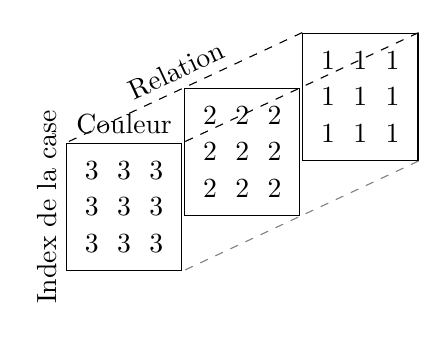
\begin{tikzpicture}
    \def\xs{1.5} %shift in x direction
    \def\ys{0.7} %shift in y direction
    \def\nm{3} % number of 2d matrices in the 3d matrix
    \foreach \x in {1,2,...,\nm}
    {
    
    \matrix [draw, % for the rectangle border
             fill=white, % so that it is not transparent
             ampersand replacement=\&] %see explanation
    (mm\x)%give the matrix a name
    at(-\x * \xs, -\x * \ys) %shift the matrix
    {
        \node {\x}; \& \node {\x}; \& \node {\x};\\
        \node {\x}; \& \node {\x}; \& \node {\x};\\
        \node {\x}; \& \node {\x}; \& \node {\x};\\
    };
    }
    
    \draw [dashed,black](mm1.north west) -- node[sloped,above] {Relation} (mm\nm.north west);
    \draw [dashed,black](mm1.north east) -- (mm\nm.north east);
    \draw [dashed,gray](mm1.south east) -- (mm\nm.south east);

    \node [rotate=90][above] at (mm3.west) {Index de la case};
    \node [above] at (mm3.north) {Couleur};
    
\end{tikzpicture}


